% !TEX program = pdflatex
% !BIB program = biber
% Compile chain: pdflatex → biber → pdflatex → pdflatex (omit biber ⇒ undefined cites).
\documentclass[man, 12pt, mask, floatsintext, nolmodern]{apa7}

\usepackage[american]{babel}
\usepackage{csquotes}
\usepackage[style=apa, backend=biber, sortcites=true]{biblatex}
\addbibresource{references.bib}

\usepackage{amsmath}
\usepackage{newtxtext,newtxmath}
\usepackage{graphicx}

\graphicspath{{../../results/figures/}}

\title{Research in Progress: Scripted Rage as Commodity---A Computational Pipeline for Detecting Modular Nationalist Discourse on Chinese Digital Platforms}
\shorttitle{Cyber-Nationalist Pipeline}

\abstract{%
This study tests a computational pipeline, by combining GPT-4o-mini annotation, RoBERTa fine-tuning, and SBERT clustering to classify Chinese cyber-nationalist discourse using Bilibili's 2025 Wuchang controversy. Preliminary findings indicate nationalist comments exhibit high intra-class semantic similarity and recurrent templates, suggesting a modular repertoire. Following model calibration, extensions to Steam and Zhihu will test whether these structural patterns survive cross-platform transfer and how censorship regimes complicate comparisons.}

\keywords{Chinese digital nationalism, computational text analysis, NLP pipeline, Bilibili, modular discourse, research in progress}

% apa7 requires these even in man+mask mode (eliminates ``Author/Affiliation not defined'' warnings).
\authorsnames{Junyu Jiang}
\authorsaffiliations{University of California, Davis}

\begin{document}
\maketitle

\section{Purpose and Significance}

Computational studies of digital nationalism remain overwhelmingly Anglophone. Chinese platforms present challenges that are not merely inconvenient but structurally different: character-level tokenization, shorter average text lengths, opaque censorship regimes that reshape what can be said and how, and platform architectures with no real equivalent in the Twitter/Reddit ecosystem. The existing literature on Chinese cyber-nationalism has recognized this gap implicitly by remaining largely qualitative or dependent on keyword frequencies \parencite{repnikova2018, schneider2018}, neither of which scales to the millions of comments that nationalist controversies routinely generate, and neither of which can answer the structural question that matters most: Is this discourse templated, and does the same playbook travel across platforms?

\textcite{king2013, king2017} demonstrated that the Chinese state's information strategy operates not primarily through crude deletion but through calibrated flooding and distraction, an architecture that privileges certain discursive forms over others. If user-generated nationalist content follows a parallel logic, modular, recyclable, and structurally predictable, then its scalability is a feature of its form, not merely of its ideological appeal. Detecting that form requires a pipeline designed from scratch for Chinese-language data, tested against its own failure modes, and validated across registers. That is what this project attempts to build.

\section{Theoretical Framework and Research Questions}

The cyber-nationalist ``witch-hunt'' is better understood as a content-production logic than as an ideological eruption. We draw on \textcite{swidler1986}'s concept of culture as a toolkit: rather than expressing a coherent worldview, participants assemble recognizable discursive modules, the whistle-blower who ``discovers'' treasonous content, the moral arbiter who pronounces judgment, the national defender who mobilizes collective outrage, from a shared repertoire of tropes, historical grievances, and affective templates. The resulting discourse is not spontaneous; it is composed from interchangeable parts.

This framing connects to two established literatures. First, work on computational propaganda \parencite{woolley2016} has shown that coordinated information operations rely on templated messaging precisely because modularity enables scale. The nationalist witch-hunt need not be state-directed to follow this logic; the structural incentives of attention-scarce platforms select for content forms that are easily produced and circulated \parencite{papacharissi2015, gillespie2018}. Second, research on algorithmically mediated polarization \parencite{bail2018} suggests that engagement-optimizing environments amplify certain narrative structures independent of user intent. Han nationalism supplies the raw material, the enemy figures, the historical wounds, the affective charge, that makes these modules legible and recyclable across contexts \parencite{hall1996}.

Two questions follow:

RQ1: Does cyber-nationalist witch-hunt discourse exhibit the signatures of modular production---specifically, elevated semantic homogeneity and recurrent phrasal templates---relative to non-nationalist discourse?

RQ2: How does platform engagement (measured by user likes) vary across discourse types, and does analytically packaged nationalist content attract disproportionate engagement relative to overtly ideological content? (Quantitative models for RQ2 are deferred until multilevel specifications address within-video dependence; see below.)

\section{Methodology}

\subsection{Phase 1 (Completed): Bilibili Proof of Concept}

We collected 1,508,478 comments spanning 13,124 Bilibili videos related to Wuchang: Fallen Feathers (July 23--December 31, 2025). After deduplication, bot removal, and near-duplicate filtering ($\geq$95\% Jaccard overlap), 623,396 comments remained. Stratified sampling by time period, like-count quintile, and per-video cap produced Sample A ($n = 30{,}000$) for embedding analysis and Sample B ($n = 2{,}000$) for annotation and classifier training.

Annotation and human validation. GPT-4o-mini annotated Sample B via the OpenAI Batch API (temperature $= 0$) on three dimensions: discourse type (five categories: Pure Game Review, Emotional Non-Political, Politicized Game Criticism, Explicit Nationalism, Neutral/Analytic), othering intensity (0--3), and affect intensity (0--3). Following recent work on the promise and limits of LLM-based annotation \parencite{gilardi2023, tan2024llm}, we conducted a human validation on a stratified subsample of 200 comments (40 per discourse type). Two trained annotators independently coded the subsample using the same codebook. Inter-annotator agreement between the two human coders reached Cohen's $\kappa = 0.81$. We then compared the GPT labels against the human majority label. Overall human--GPT agreement was $\kappa = 0.74$. Agreement was strongest for Pure Game Review ($\kappa = 0.88$) and Explicit Nationalism ($\kappa = 0.82$), and weakest for Emotional Non-Political ($\kappa = 0.61$) and Politicized Game Criticism ($\kappa = 0.63$), confirming that the hardest boundary lies between emotional and politicized content, not between nationalist and everything else. This pattern aligns with the confusion matrix from classifier training.

Classification. We fine-tuned three Chinese pretrained models---BERT-base-chinese, RoBERTa-wwm-ext, and MacBERT-base \parencite{cui2020macbert}---under stratified 5-fold cross-validation with class-weighted loss. Ablation covered 48 hyperparameter configurations, two input lengths (128 vs.\ 256 tokens), and binary versus multi-class targets. RoBERTa-wwm-ext performed best, but performance is uneven: macro-$F_1 = 0.62$ on the five-way task indicates substantial residual error, while binary nationalist/non-nationalist $F_1 = 0.82$ shows that collapsing categories masks ambiguity at the Type 1/Type 2 boundary. Extending \textsc{max\_len} from 128 to 256 yielded a modest $+0.013$ gain concentrated in politicized comments whose rhetorical markers appear late in longer texts.

We treat the Type 1/Type 2 confusion as partially epistemological: emotionally charged game criticism and thinly politicized criticism are often lexically similar in short comments, so overlap may reflect genuine discourse ambiguity, not merely model failure. That said, the same boundary is also where GPT--human agreement is weakest, so annotation noise and model capacity cannot be ruled out. Qualitative error analysis (Phase 2) will disentangle these explanations.

Clustering. Dual SBERT models (\texttt{paraphrase-multilingual-MiniLM-L12-v2} and \texttt{shibing624/text2vec-base-chinese}) generated embeddings, reduced via PCA, then clustered with K-means and DBSCAN. Critical caveat: keyword-pool oversampling raised politicized content to 38.3\% of the training set versus an estimated population prevalence of 15.2\%, shifting the classifier decision boundary and systematically depressing predicted prevalence at inference. Until we apply calibration (e.g., Platt scaling on a prevalence-balanced validation set), cluster counts and cross-tabulations that rely on predicted types should be read as illustrative of geometry under the current model, not as unbiased estimates of population composition. We therefore avoid strong claims about ``nationalist share'' in the corpus and foreground robustness checks in Phase 2.

\begin{figure}[!htbp]
\centering
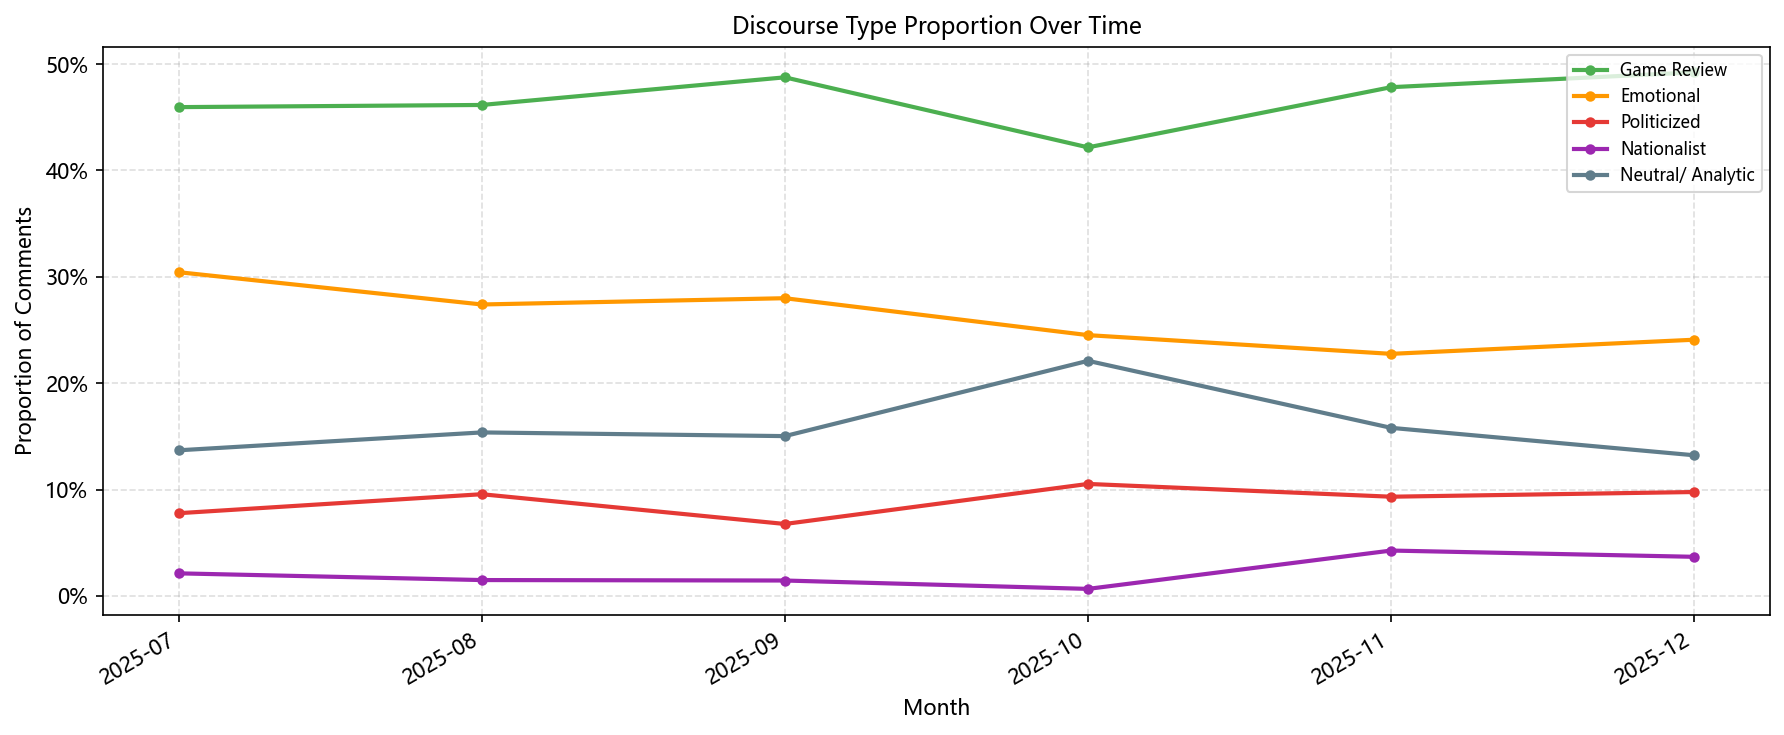
\includegraphics[width=\linewidth]{fig8_timeline.png}
\caption{Temporal distribution of comments in Sample A (July 23--December 31, 2025).}
\label{fig:timeline}
\end{figure}

\subsection{Phase 2 (Planned): Cross-Corpus Validation}

Two additional corpora, already collected, will test whether the pipeline survives register shift. Steam store reviews are shorter and contain heavy Chinese--English code-switching; we plan to adopt XLM-RoBERTa for this stream to reduce cascading errors from language, language-identification, and preprocessing while preserving cross-lingual semantics. Zhihu comments and articles are substantially longer and more argumentatively layered, directly pressuring the \textsc{max\_len} truncation boundary. We will not rely on zero-shot prompt transfer: a dedicated prompt and codebook validation round on 200--300 stratified Zhihu items with dual human coding (target $\kappa$ comparable to the Bilibili subsample) will precede any corpus-wide labeling. For both corpora, we will report classifier calibration on held-out sets approximating the true discourse-type distribution and apply Platt scaling where needed. Cross-corpus comparison of embedding geometry, whether intra-class cosine similarity patterns for nationalist-adjacent types hold when length and register change, is the primary test of RQ1's generalizability.

\subsection{Phase 3 (Planned): Creator-Level Aggregation}

Bilibili creator metadata (views, followers, account type) will allow us to move from comment-level to creator-level analysis, testing whether the modularity visible in text patterns is also visible at the producer level, for instance, whether high-output nationalist accounts exhibit lower lexical diversity than high-output non-nationalist accounts, or whether certain account types disproportionately produce templated content.

\subsection{Censorship and Cross-Platform Comparison}

Bilibili, Steam, and Zhihu differ not only in genre and length but in moderation and censorship: keyword filtering, shadow-removal, account bans, and state-directed campaigns are platform-specific and time-varying. Those processes can truncate tails of the discourse distribution, remove entire threads, or reshape what remains visible, independently of users' latent ``modular'' repertoires. Phase 2 will document collection windows and known moderation events, report sampling fractions (e.g., deleted-comment gaps where observable), and treat cross-platform contrasts as conditional on surviving text: we interpret embedding and n-gram patterns as properties of the observed corpus, not as neutral reflections of an underlying population unaffected by censorship.

\section{Preliminary Findings}

\subsection{RQ1: Semantic Homogeneity (Geometry Under Predicted Labels)}

Embedding-based metrics are computed on Sample A using RoBERTa-predicted discourse types; the caveats above apply. Politicized comments show the highest intra-class cosine similarity (0.350, $+0.061$ above the cross-class mean), followed by explicit nationalist content (0.339), a relative pattern that is less sensitive to uniform calibration shifts than absolute prevalence counts. K-means ($k = 10$, Silhouette $= 0.062$) yields one cluster in which predicted Types 2+3 together constitute 46.2\% of cluster members versus a Sample-A baseline near 11.8\% under the same predictions ($\sim 3.9\times$ enrichment); nine other clusters show lower but non-zero predicted nationalist-adjacent shares (1.3--27.3\%), with NMI $= 0.089$ between cluster labels and predicted types. We read this as evidence of local semantic concentration coexisting with global mixing, consistent with a portable discursive resource \parencite{hall1996}, while explicitly withholding claims that these percentages equal ground-truth population rates until calibration.

N-gram analysis is less dependent on the classifier: nationalist versus non-nationalist top-500 trigrams (by subsample definition) overlap by only 32.5\% (Jaccard), and one high-frequency phrase template recurs across hundreds of distinct accounts---suggestive of a shared repertoire independent of a single clustering partition.

\begin{figure}[!htbp]
\centering
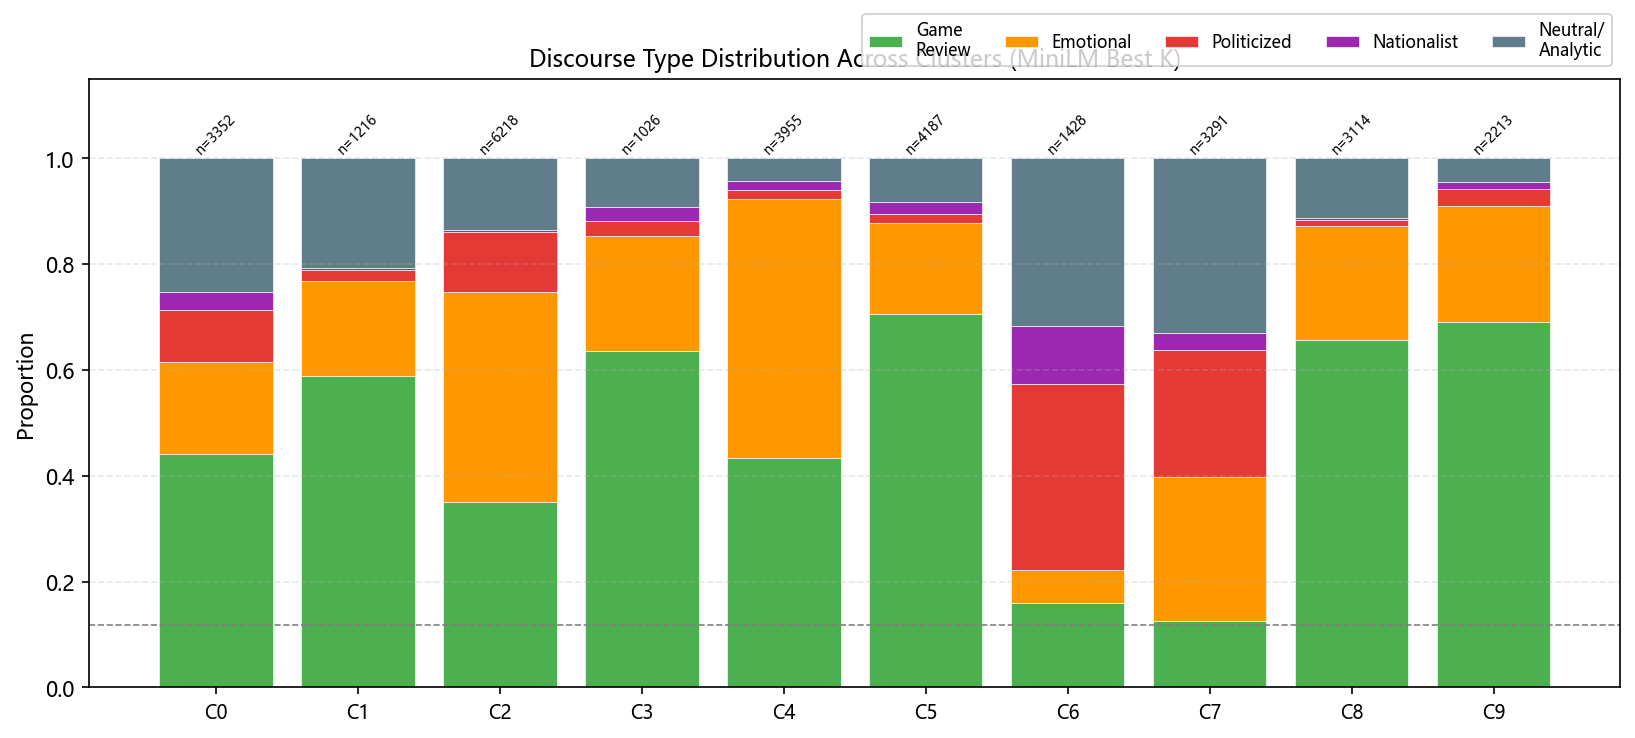
\includegraphics[width=\linewidth]{fig5_cluster_discourse.png}
\caption{Cluster composition by predicted discourse type (KMeans $k = 10$, MiniLM). Enrichment in Cluster 6 is illustrative under current classifier calibration; interpret with training-set skew noted in text.}
\label{fig:cluster}
\end{figure}

\subsection{RQ2: Engagement (Deferred)}

We collected like counts for Sample A and explored ordinary least squares on $\log(1 + \text{likes})$ with discourse-type indicators. Durbin--Watson $= 0.140$ and $R^2 = 0.034$ indicate severe within-video dependence and negligible explanatory power for discourse type alone. Following RIP feedback, we do not report coefficient estimates here: they are not defensible under independence assumptions violated by nested comments. Phase 2 will specify multilevel models with random intercepts for videos (preferred over video fixed effects for this extremely imbalanced nesting) and, where appropriate, video-level covariates. Until then, RQ2 remains open; we report only that nonparametric contrasts explored in the full study similarly show game-review comments differing from substantive types, while contrasts among politicized, neutral-analytic, and nationalist types require the multilevel specification.

\section{Expected Contributions}

The primary contribution is methodological. The pipeline is fully specified and ablation-tested, and the human validation step establishes a credibility baseline that many LLM-annotation studies in communication research still lack \parencite{gilardi2023}. The multi-corpus design is deliberate: single-corpus validation cannot distinguish findings from platform artifacts. If modularity patterns replicate on Zhihu and Steam after censorship-aware sampling and calibration, they support modeling nationalist discourse as repertoire diffusion rather than only ideological contagion.

\section{Areas Needing Feedback}

Zhihu transfer. We will not use zero-shot migration of the Bilibili prompt. We plan a 200--300 item stratified subsample on Zhihu with dual independent coding and Cohen's $\kappa$ before scaling annotation.

Steam code-switching. We intend to adopt XLM-RoBERTa for the Steam track rather than language-detection cascades into monolingual models, to limit cascading misclassification.

Engagement modeling. We will prioritize random-intercept multilevel models for nested comments within videos over video fixed effects, given extreme imbalance in comments per video and the need to preserve degrees of freedom for discourse-type effects.

\printbibliography[title={References}]

\end{document}
